\documentclass{article}
\usepackage[superscript,biblabel]{cite}
\usepackage{graphicx}
\usepackage{float}

\graphicspath{{../../analysis/images/}}
\bibliographystyle{naturemag}

\title{Epistasis is widespread in the genetic control of transcription in humans}
\date{}
\author{Gibran Hemani, Konstantin Shakhbazov, Joseph E Powell}

\begin{document}

\maketitle


\begin{abstract}
A long standing question in evolution and human genetics is the extent to which epistasis, the phenomenon whereby one polymorphism's effect on a trait depends on other polymorphisms present in the genome, contributes to complex traits \cite{Carlborg2004, Hill2008a, Crow2010}. Though epistasis has been demonstrated in artificial gene manipulation studies in model organisms \cite{Costanzo2010, Bloom2013}, and some examples have been shown in other species \cite{Carlborg2006}, few convincing examples exist for epistasis amongst natural polymorphisms in human traits \cite{Strange2010, Evans2011}. Its absence from empirical findings may simply be due to its unimportance in the genetic control of complex traits \cite{Hill2008a, Crow2010}, but we sought to test the hypothesis that it has previously been too technically difficult to detect due to statistical power and computational issues \cite{Cordell2009}. Here we show that, using advanced computation techniques \cite{Hemani2011} and a gene expression study design where any effects are expected to be large \cite{Powell2012}, evidence for multiple instances of epistasis is found. In a cohort of 846 individuals with data on 7339 gene expression levels in whole blood, we found that after stringent correction for multiple testing the expression of 249 genes is controlled by 549 significant pairwise epistatic interactions. We attempted replication in two independent datasets \cite{Metspalu2004, Fehrmann2011} and 421 showed evidence of significance in at least one dataset. We provide evidence of functional enrichment for the interacting SNPs, for instance 49 of the genetic interactions are located within 500kb of known chromosome interactions \cite{Lan2012} ($p < 1.1 \times 10^{-70}$). One hundred and twenty-nine genes are controlled by multi-locus epistatic interactions whereby one \emph{cis}-acting single nucleotide polymorphism (SNP) is modulated by several trans-acting SNPs. For example MBNL1 is controlled by an additive effect at rs13069559 which itself is controlled by \emph{trans}-SNPs on 14 different chromosomes, with nearly identical genotype-phenotype (GP) maps for each \emph{cis}-\emph{trans} interaction. This study presents the first strong evidence for the widespread existence of epistatic genetic effects emerging from natural genetic variation in humans.
\end{abstract}


\section{Main text}

% \subsection{Introduction}
The past decade has seen a tremendous amount of activity in mapping genetic polymorphisms that underlie complex traits. Typically, SNPs are treated as contributing linearly, independently, and cumulatively to the mean of a trait and this has been successful in identifying thousands of causal variants \cite{Visscher2012}. Yet outside the prism of association studies there is widespread evidence for epistasis, not only at the molecular scale in artificial double gene knockouts in experimental organisms \cite{Costanzo2010} but also at the evolutionary scale in fitness adaptation \cite{Weinreich2006} and speciation \cite{Breen2012}. Though its importance is frequently the subject of debate \cite{Carlborg2004, Hill2008a, Crow2010}, to date there is little convincing empirical evidence for epistasis playing a substantial role in the architecture of complex traits in humans \cite{Strange2010, Evans2011}.

Detection of epistasis is hampered by power issues for several reasons, including increased dependence on linkage disequilibrium (LD) between causal SNPs and observed SNPs \cite{Weir2008, Hemani2013}, increased model complexity in fitting interaction terms \cite{Marchini2005}, and more extreme significance thresholds to account for increased multiple testing \cite{Cordell2009}. When genetic effect sizes are small, as is expected in most complex traits of interest \cite{Visscher2012}, the power to detect epistasis diminishes rapidly. There are two ways to overcome this problem, either by using extremely large sample sizes \cite{LangoAllen2010}, or use traits that are likely to have large effect sizes. Because our focus was to ascertain the extent to which epistasis exists amongst natural genetic variation we opted for the latter approach and searched for epistasis controlling gene expression levels. Transcription levels can be measured for thousands of genes and these traits are largely heritable but on average less polygenic than high level phenotypes \cite{Powell2013}, thus it is expected that any genetic effects will be relatively large, maximising the chance at detecting epistasis should it exist.


% \subsection{Initial search in discovery set}
We searched for pairwise epistasis exhaustively in the Brisbane Systems Genetics Study (BSGS) dataset \cite{Powell2012}, which comprises 846 individuals who are genotyped at 528509 autosomal SNPs and who have gene expression levels measured in whole blood samples for 7339 probes representing 6158 RefSeq genes. Recent hardware and software \cite{Hemani2011} advances made it possible to perform the $1.03 \times 10^{15}$ statistical tests to complete this analysis. We used permutation analysis \cite{Churchill1994a} to calculate an experiment-wide significance threshold of $2.91 \times 10^{-16}$ at the 5\% family-wise error rate (FWER). SNP pairs were modelled for full genetic effects, including marginal additive and dominance at both SNPs plus four interaction terms. Though we could have used a less complex model to improve statistical efficiency, we deemed it important to be agnostic about the type of epistasis that might exist, and therefore chose not to over-parameterise the test \cite{Marchini2005, Hemani2013}. Because there are many large marginal effects present in these data it was necessary to perform several filtering steps to exclude SNP pairs that were significant due to marginal effects alone. All SNP pairs with LD $r^2 > 0.1$ were removed, and were required to have at least five data points in all nine genotype classes. If multiple SNP pairs were present on the same chromosomes for a particular expression trait then only the sentinal SNP pair was retained. Finally, a nested test contrasting the full genetic model against the marginal additive and dominance model was performed for each remaining SNP pair (Methods), resulting in 549 significant interactions after Bonferroni correction for multiple testing of the filtered SNPs.


% \subsection{Replication}
Though a necessary step to establish the veracity of the signals from the discovery set, it is theoretically difficult to replicate epistasis because the dependence on LD between observed SNPs and causal variants is on average four orders of magnitude higher than it is for independent additive effects \cite{Weir2008, Hemani2013}. The significant SNP pairs were carried forward for replication in two independent datasets that used the same expression assays for analysing transcription in whole blood, the Fehrmann dataset \cite{Fehrmann2011} ($n=1240$) and the Estonian Genome Centre University of the University of Tartu (EGCUT) dataset \cite{Metspalu2004} ($n=891$). We observed substantial replication of interaction signals in both datasets. Of the 480 original pairs that passed filtering (Methods) in Fehrmann and EGCUT, 421 of the SNP pairs showed replication for the interaction test at the 5\% false discovery rate (FDR) level in at least one dataset, and 148 in both datasets (Supplementary Figure \ref{fig:qqplotfdr}). The congruence of the epistatic networks in discovery and replication datasets is shown in Figure \ref{fig:fireworks}, demonstrating that these complex genetic patterns are common even across independent populations. We also report that 39 of the interactions from the discovery set were significant at the Bonferroni level in at least one replication set (Supplementary Figure \ref{fig:qqplotbonf}), and 18 were significant in both. The GP maps for these interactions are remarkably similar in all three datasets (Figure \ref{fig:gpmaps}). A further replication was attempted using the Centre for Health Discovery and Wellbeing (CHDWB) dataset \cite{Preininger2013}, but only 185 of the SNP pairs passed filtering because the sample size was small ($n=139$), and due to insufficient power we found no evidence for replication.


% \subsection{Patterns of epistasis}
Though seldom the focus of association studies, SNPs with known main effects are often tested for additive $\times$ additive genetic interactions \cite{Cordell2009}, but our analysis shows this is unlikely to be the most effective framework for its detection. The majority of interactions comprised of one SNP that had a previously known association and one that had no previous association in the dataset \cite{Powell2013} (476 out of 549). Only 9 interactions were between SNPs that both had marginal effects while 64 were between SNPs that had no known marginal effects. Additionally, we observed that the largest epistatic variance component for the 529 interactions were divided amongst additive $\times$ additive, additive $\times$ dominance and dominance $\times$ dominance terms proportional to what is expected by change ($p = 0.22$ for divergence from expectation). This is perhaps to be expected because the patterns of epistasis used for statistical decomposition are not designed to resemble biological function \cite{Cockerham1954}.

We observed a wide range of significant GP maps (Figure \ref{fig:gpmaps}) but the most common pattern of epistasis that we detected involved a \emph{trans}-SNP masking the effect of an additive \emph{cis}-SNP. For example, MBNL1 (involved in RNA modification and regulation of splicing \cite{Ho2004}) has a \emph{cis} effect at rs13069559 which in turn is controlled by 14 \emph{trans}-SNPs that exhibit a masking pattern, such that when the \emph{trans}-SNP is homozygous for the masking allele the decreasing allele of the \emph{cis}-SNP no longer has an affect. Each of these interactions have evidence for replication in at least one dataset and eight have evidence for replication in both datasets (Supplementary Figure \ref{fig:circleplots}). We observed that nine of the 14 \emph{trans} SNPs are located in intronic regions (proportion of SNP panel in introns $= 0.05$, $p = 3.11 \times 10^{-9}$), suggesting a putative mechanism by which epistatic interactions may regulate transcription.


% \subsection{Functional annotation}
Of the 549 interactions, 66 were \emph{cis}-\emph{cis} acting (both SNPs were on the same chromosome as the expression gene), 470 were \emph{cis}-\emph{trans}-acting, and 13 were \emph{trans}-\emph{trans}-acting. In total the 549 interactions comprised 835 unique SNPs, which we analysed for functional enrichment. We tested the SNPs for cell-type specific overlap with transcriptionally active chromatin regions, tagged by histone-3-lysine-4,3-methylation (H3K4me3) chromatin marks, in 34 cell types \cite{Trynka2013}. There was significant enrichment for \emph{cis}-acting SNPs in haematopoeitic cell types only ($p < 1 \times 10^{-4}$ for the three tissues with the strongest enrichment are significant at after adjusting for multiple testing, Supplementary Figure \ref{fig:transh3k4me3}). However \emph{trans}-acting SNPs did not show any tissue specific enrichment ($p > 0.1$ for all tissues, Supplementary Figure \ref{fig:transh3k4me3}). This difference between \emph{cis} and \emph{trans} SNPs suggests that there is a range of molecular mechanisms by which epistasis might arise beyond tissue specific transcription. There is also strong enrichment for SNPs to be localised in enhancer regions \cite{Ward2012a} (Supplementary Figure \ref{fig:enhancers}). This enrichment is consistent for both \emph{cis} and \emph{trans} SNPs ($p < 1 \times 10^{-6}$). In particular, there was substantial enrichment for the GATA2 binding motif within 1kb of all epistatic SNPs, a known regulator of transcription in haematopoietic cells \cite{Tsai1994} ($p = 1 \times 10^{-40}$).

We also demonstrate another putative novel mechanism by which biological function can lead to epistatic genetic variance. We cross referenced our epistatic SNPs with a map of chromosome interacting regions ($n = 96139$) in K562 blood cell lines \cite{Lan2012}. Forty-nine epistatic SNP pairs mapped to within 500kb of a chromosome interaction, and 69 mapped to within 2Mb ($p < 1.1 \times 10^{-70}$), (Supplementary Figure \ref{fig:chromosomeinteractions}), but decyphering the exact cellular processes underlying this interaction requires further research.


% \subsection{Contribution of epistatic variance}
Though we present many instances of epistasis, quantifying its relative importance to complex traits in humans remains an open question. In this study we are able to identify 249 probes with at least one significant interaction given our experiment-wide threshold. Using the same threshold ($p < 2.91 \times 10^{-16}$) for the same data but searching for only additive effects returns 517 probes out of the 7339 analysed with at least one significant expression quantitative trait locus (eQTL) \cite{Powell2012}, therefore we argue that the number of instances of epistasis are substantial. However in terms of their contribution to complex traits a more important metric might be the proportion of the variance that the epistatic loci explain \cite{Hill2008a}. Ideally one would approach this question from a whole genome level \cite{Visscher2008} but this is intractable for non-additive variance components. Yet some inference can be made from the ascertained effects in these analyses and it is evident that additive variance is overall a larger component than epistatic variance as has been argued previously \cite{Hill2008a, Crow2010}. We observe that of the significant interactions detected the average additive contribution to the total detected genetic variance is 72.7\%, over three times higher than the epistatic contribution of 24.1\% (Figure \ref{fig:variancecomponents}).

From an experiment-wide perspective, the proportion of the total phenotypic variance for all 7339 probes explained by additive effects significant at the $p < 2.91 \times 10^{-16}$ threshold, as reported in an independent study on the same dataset that focused on additive effects only \cite{Powell2012}, is 1.9\%. In contrast, the epistatic signals detected in this study explains 0.27\%, approximately seven times lower than the additive variance. There are two caveats to this comparison, firstly the power of a 1 \emph{d.f.} test exceeds that of an 8 \emph{d.f.} test. Secondly the non-additive variance at causal variants is expected to be grossly underestimated by observed SNPs in comparison to estimates for additive variance \cite{Weir2008, Hemani2013}, due to differences in the rate of decay estiamted variance between observed and causal SNPs as LD decreases. Therefore this is likely to be a lower bound on the estimate of the relative contribution of epistasis.


% \subsection{Discussion}
Overall, we have demonstrated that it is possible to identify and replicate epistasis in complex traits amongst common human variants. The functional analysis of the significant epistatic loci suggests that there are a large number of possible mechanisms that can lead to non-additive genetic variation, thus it is not surprising that instances of epistasis should be widespread. Further research into such genetic effects may provide a useful portal to understanding molecular mechanisms with greater clarity. With data and computational techniques now widely available the search for epistasis in larger datasets for traits of broader interest is warranted.



\clearpage
\section{Figures}

\begin{figure}[H]
	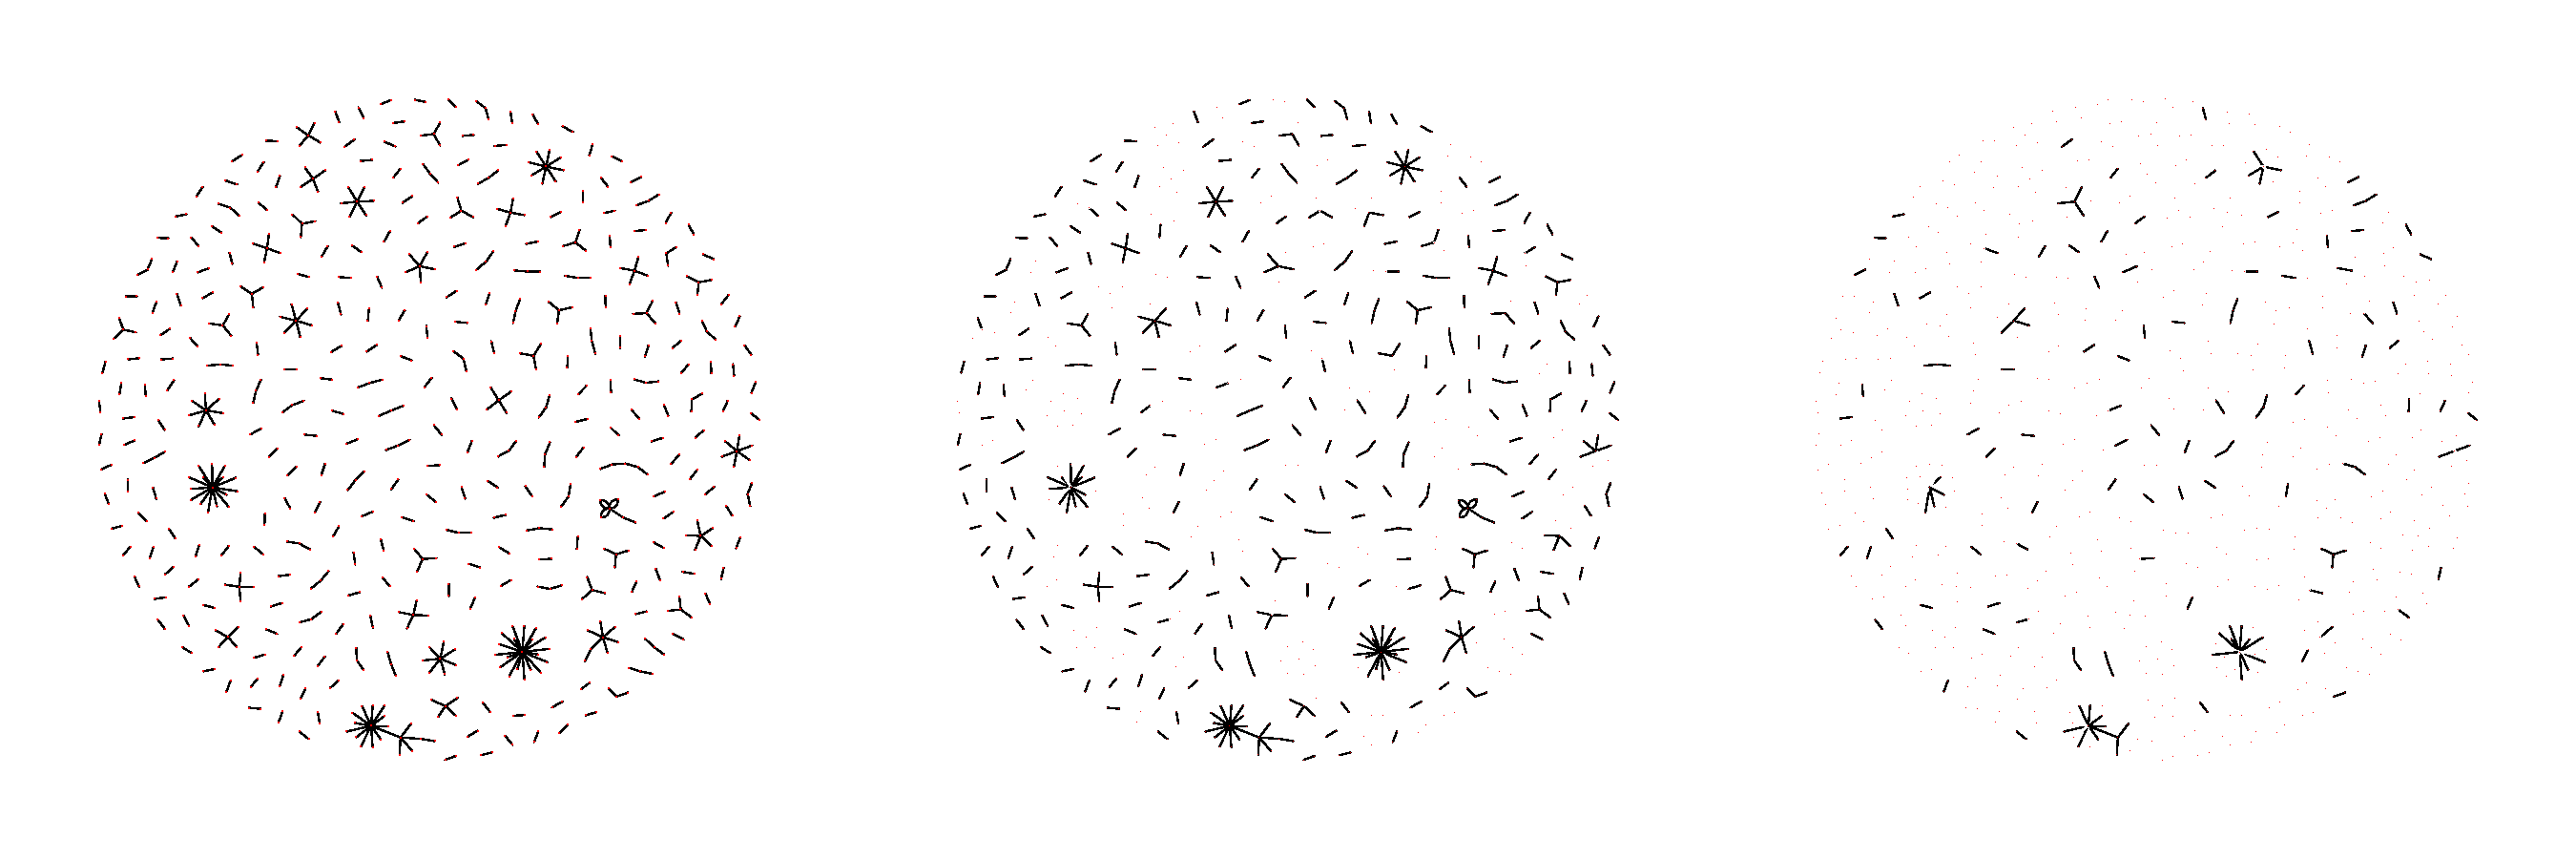
\includegraphics[width=5in]{hairballs_all_reps.pdf}
	\caption{\textbf{Replication of epistatic networks in two cohorts} Panel A represents all 549 genetic interactions (edges) discovered in the discovery set. Panel B shows those interactions that were present at the 5\% FDR level in at least one replication dataset, and panel C shows which interactions were significant in both replication datasets. Red nodes represent probes and black nodes represent SNPs. The congruence between datasets is indicitive of the consistent epistatic instances in independent populations.}
	\label{fig:fireworks}
\end{figure}
\clearpage

\begin{figure}[H]
	\includegraphics[width=5in]{gpbonfrep.pdf}
	\caption{\textbf{Replication of genotype-phenotype (GP) maps in two cohorts} The GP maps for each epistatic interaction that is significant at the Bonferroni level in both replication datasets are shown. Each tile represents the expression level for that two-locus genotype class. Phenotypes are for gene transcript levels, where the gene symbol is labelled in the panel columns. Panel rows are labelled for the dataset. Phenotypes for each interaction within each cohort are scaled to be between 0 and 1. There is a general trend of the GP maps replicating across all three datasets.}
	\label{fig:gpmaps}
\end{figure}
\clearpage

\begin{figure}[H]
	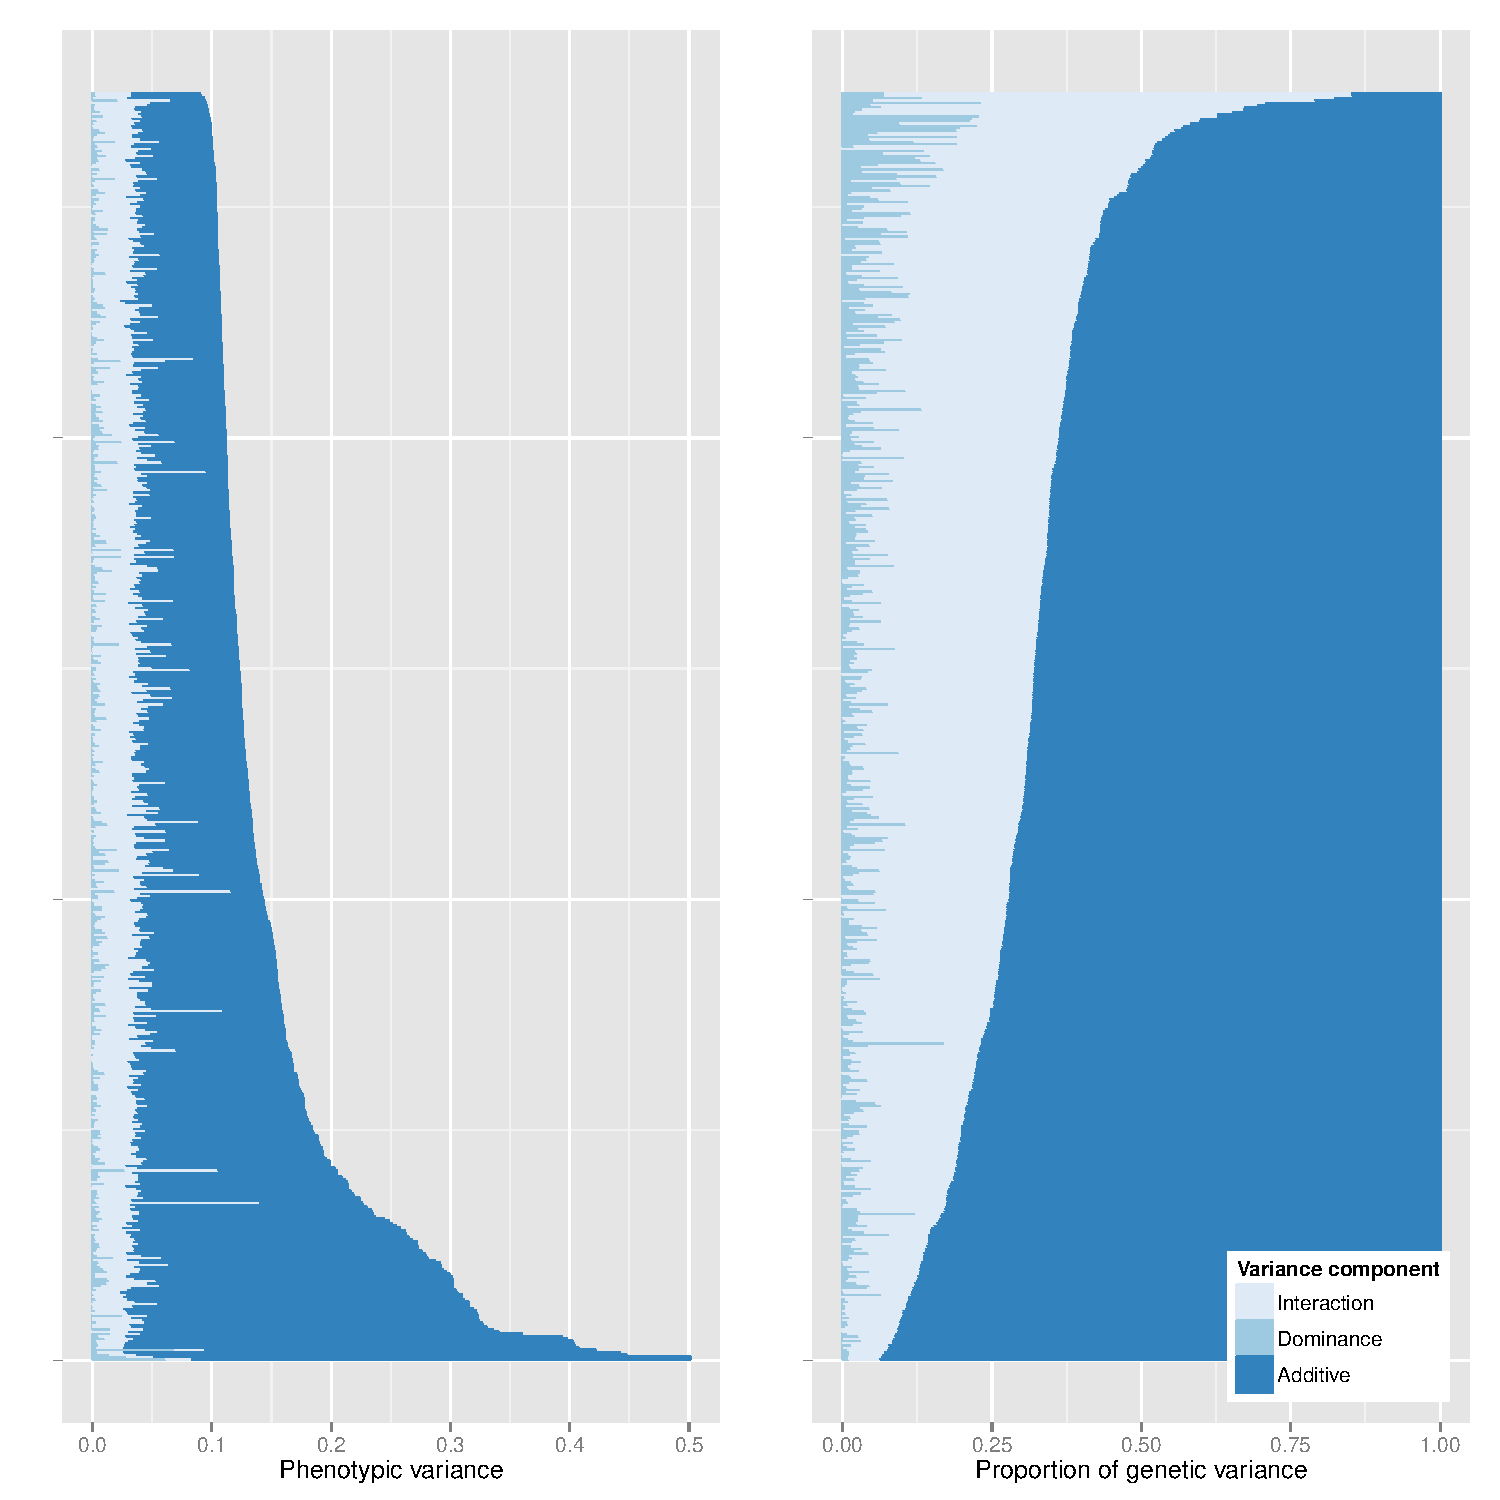
\includegraphics[width=5in]{variance_components.pdf}
	\caption{\textbf{Comparison of genetic variances} Panel A shows the proportion of phenotypic variation ($x$-axis) that is captured by additive, dominant and interaction components for all 529 significant interactions, ordered by total phenotypic variance explained by the SNP pair along the $y$-axis. Panel B shows the proportion of the genetic variance ($x$-axis) that is attributable to the three variance components, ordered by the proportion that is additive.}
	\label{fig:variancecomponents}
\end{figure}
\clearpage


% \clearpage
% \section{Figures}
% \setcounter{figure}{0}

% \begin{figure}[H]
% 	\centering
% 	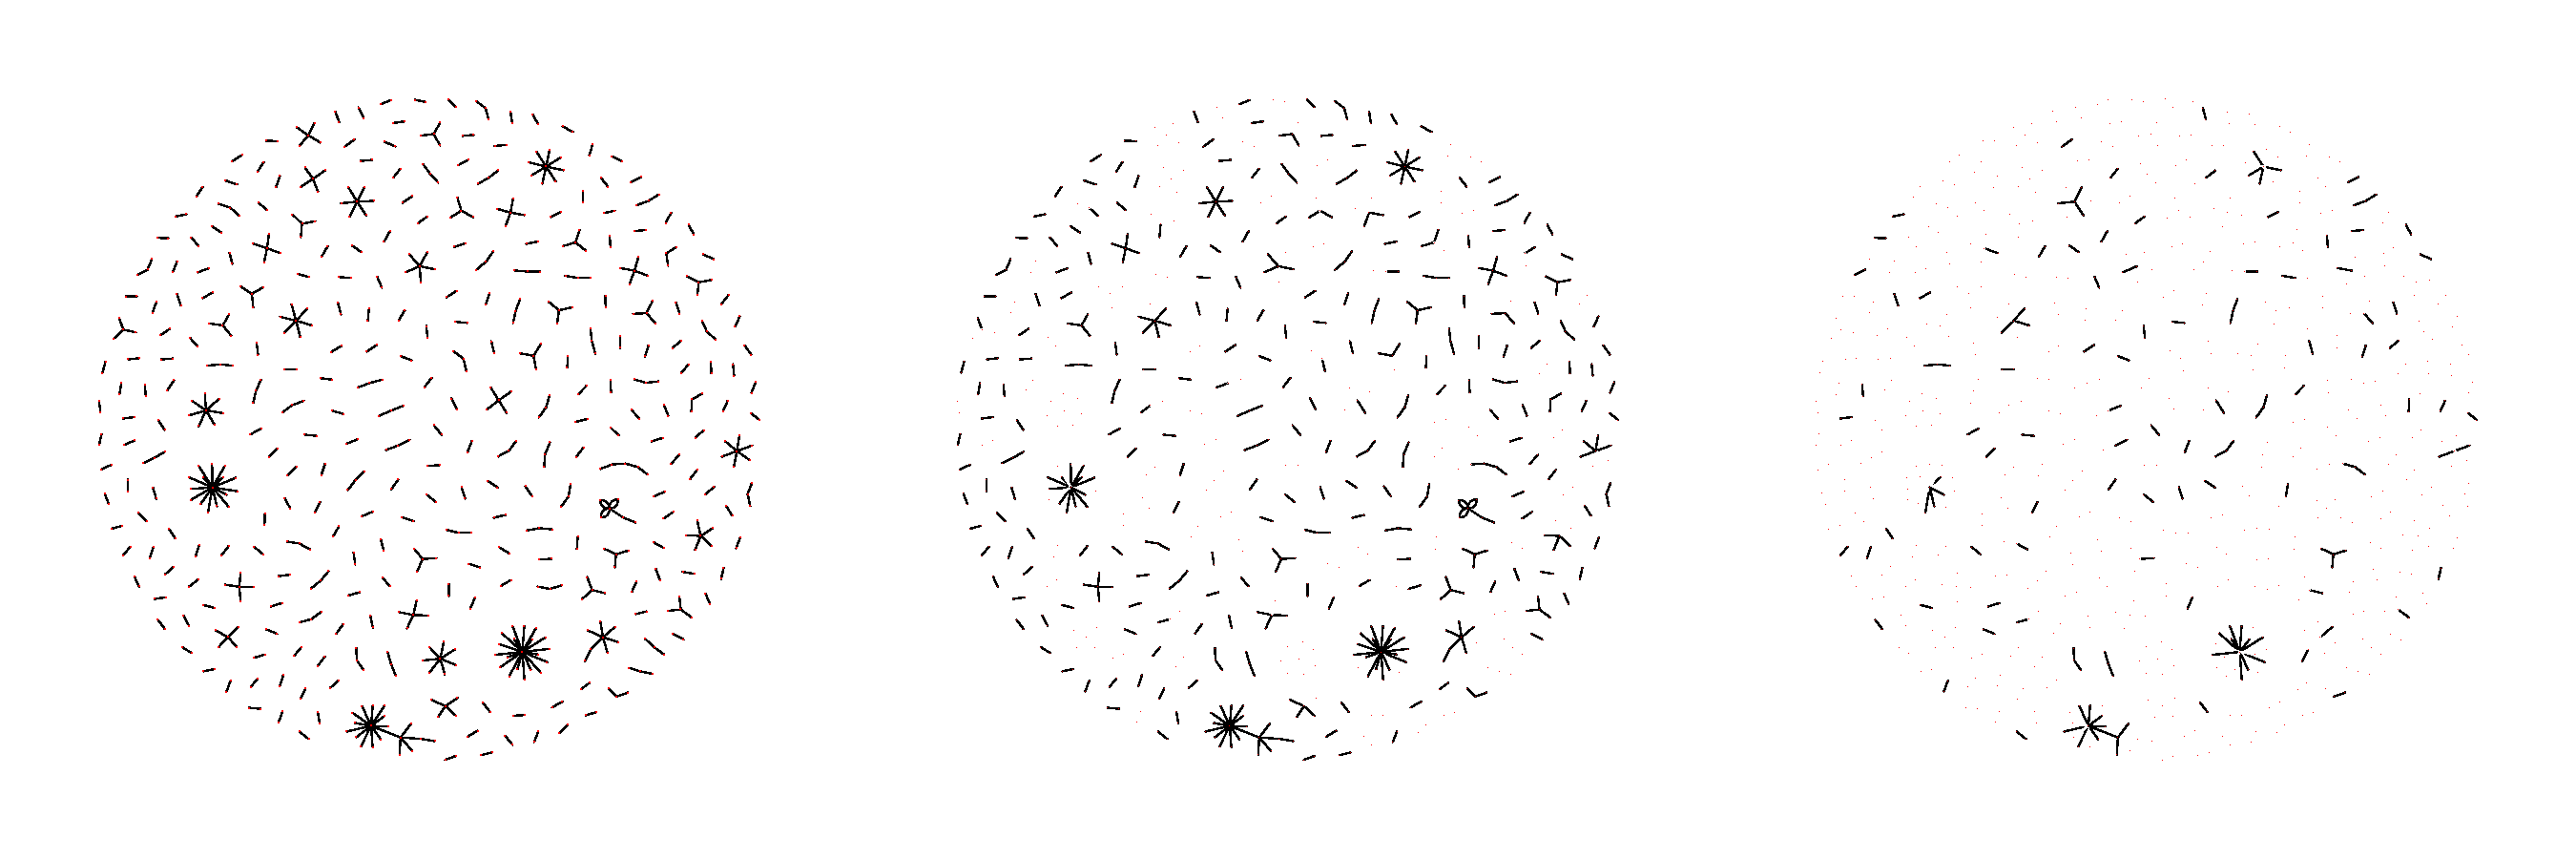
\includegraphics[width=5in]{hairballs_all_reps.pdf}
% 	\caption{}
% \end{figure}
% \clearpage

% \begin{figure}
% 	\centering
% 	\includegraphics[width=5in]{gpbonfrep.pdf}
% 	\caption{}
% \end{figure}
% \clearpage

% \begin{figure}
% 	\centering
% 	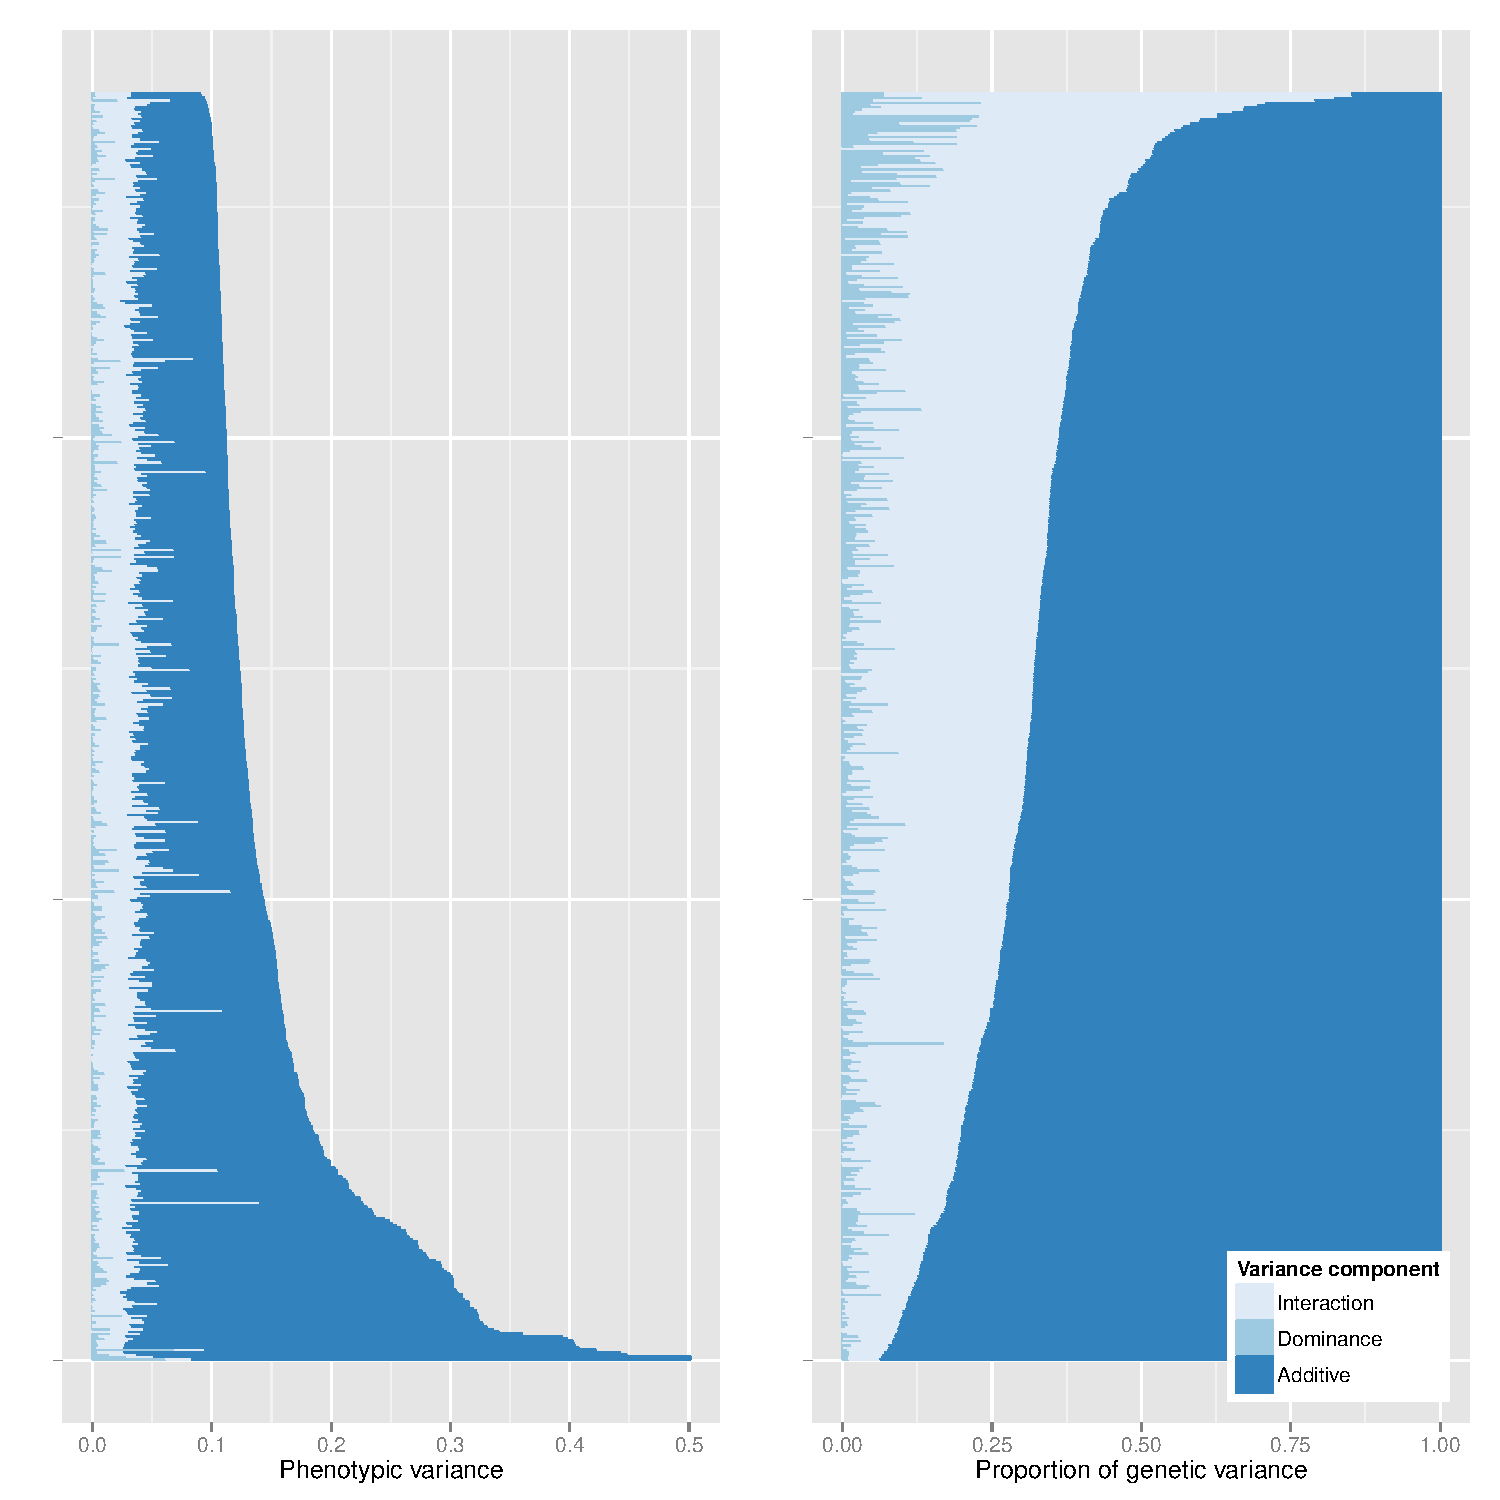
\includegraphics[width=5in]{variance_components.pdf}
% 	\caption{}
% \end{figure}


\clearpage
\section{Supplementary Figures}
\setcounter{figure}{0}
\makeatletter 
\renewcommand{\thefigure}{S\@arabic\c@figure} 
\makeatletter 

\begin{figure}[H]
	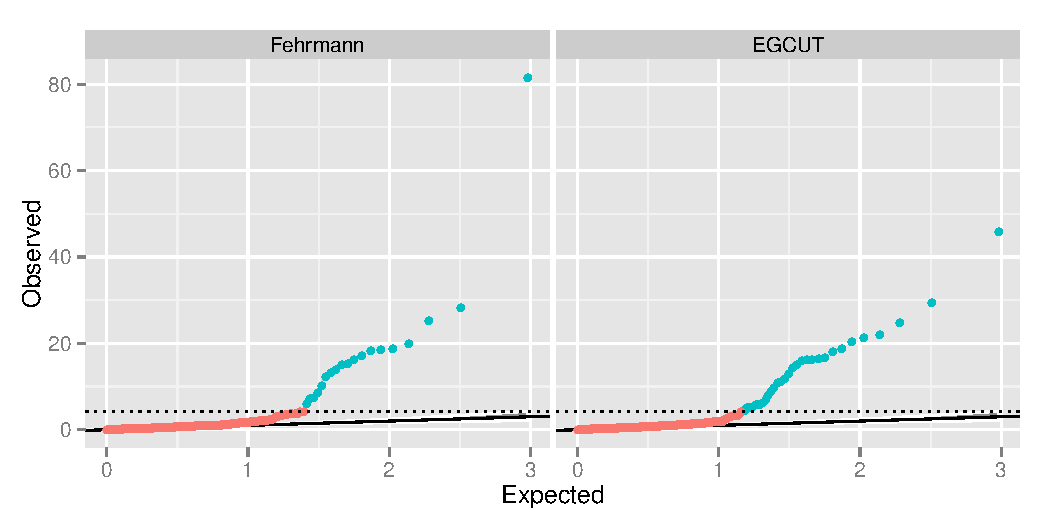
\includegraphics[width=5in]{qqbonf}
	\caption{\textbf{Q-Q plots of interaction $p$-values in two independent datasets} Of the 549 discovery interactions, interaction $p$-values (4 \emph{d.f.} test) were obtained for 480 SNP pairs that passed filtering in the two replication datasets. The $p$-values plotted along the $y$-axis, and the expected $p$-values are plotted along the $x$-axis. Green points represent $p$-values that surpass Bonferroni correction.}
	\label{fig:qqplotbonf}
\end{figure}
\clearpage

\begin{figure}
	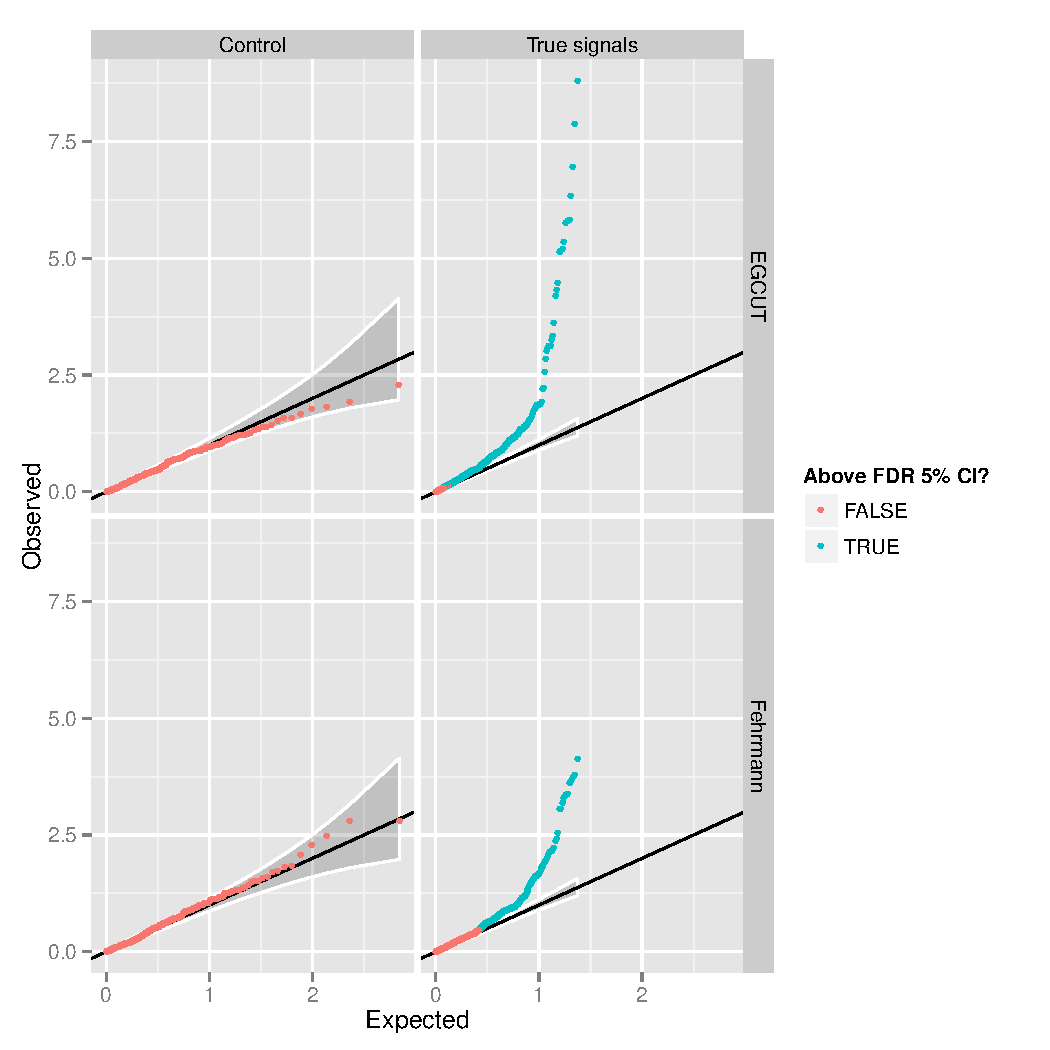
\includegraphics[width=5in]{qqfdr}
	\caption{\textbf{Q-Q plots of replicated interaction $p$-values excluding the 20 most extreme $p$-values} The left panel (Null) shows the replication $p$-values from 549 randomly drawn SNP pairs in the Fehrmann (top row) and EGCUT (bottom row) datasets. The right panel (Observed) shows the interaction $p$-values from the 460 least significant pairs that pass filtering in the two replication datasets (\emph{i.e.} excluding the 20 most extreme $p$-values for clarity). Dark blue points represent $p$-values that surpass the 5\% FDR level.}
\label{fig:qqplotfdr}
\end{figure}
\clearpage

\begin{figure}
	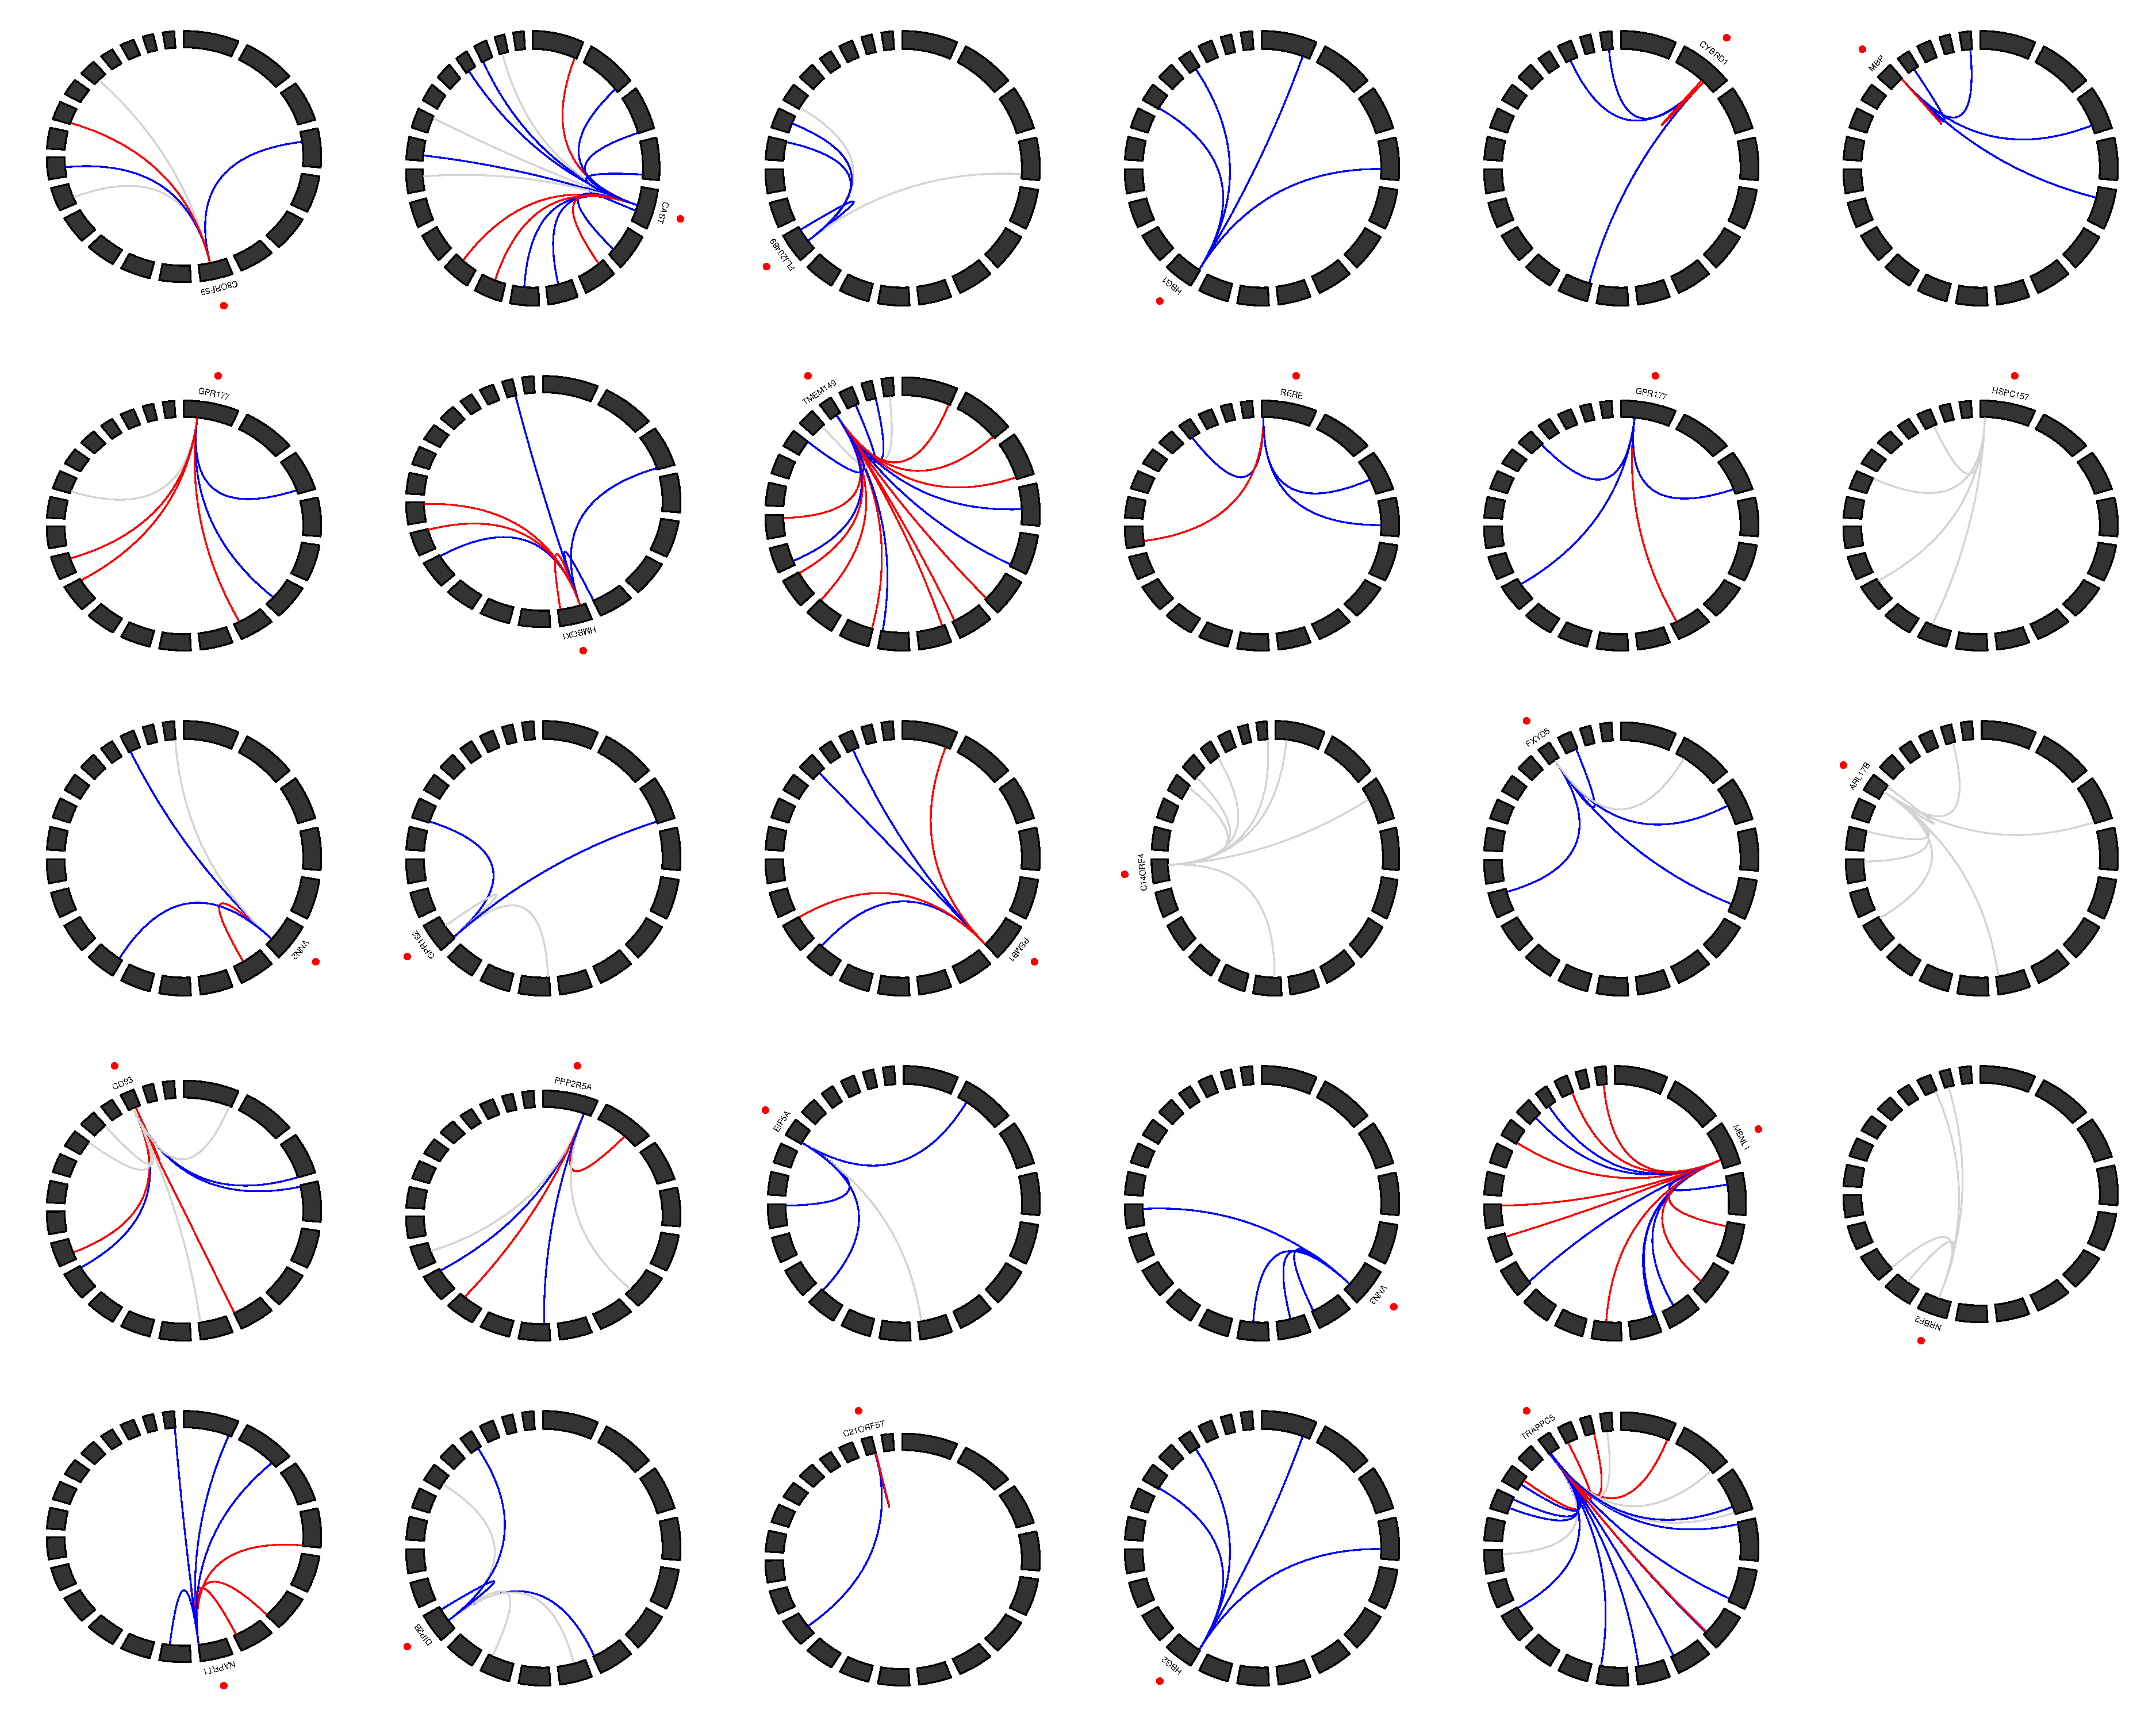
\includegraphics[width=5in]{circles_replication2}
	\caption{\textbf{Gene expression traits with four or more genetic interactions} Circle plots represent the genomic positions for SNPs (linking lines) and expression probes (red points). Chromosomes are represented by black blocks and ordered from 1 to 22 clockwise, starting from the top. Grey lines represent no evidence for replication, blue lines denote replication in at least one dataset, and red lines denote replication in two datasets. Most interactions are characterised as being \emph{cis}-\emph{trans} to the expression probe.}
	\label{fig:circleplots}
\end{figure}
\clearpage

\begin{figure}
	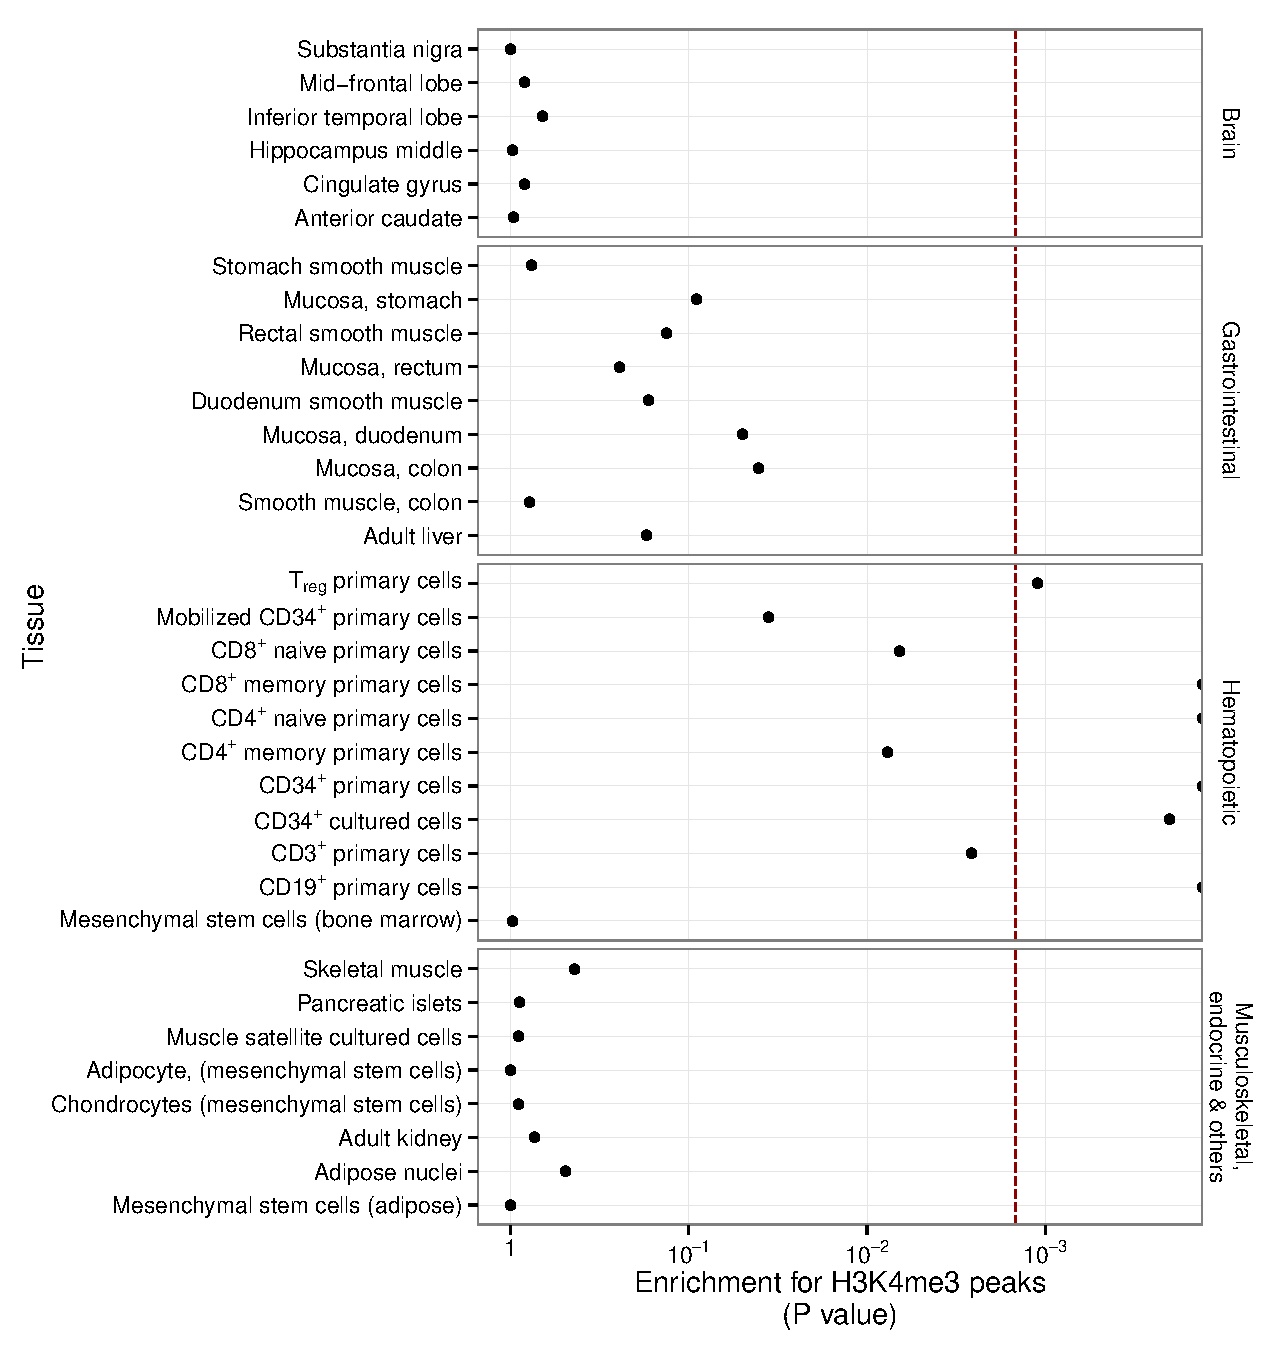
\includegraphics[width=5in]{cis_h3k4me3}
	\caption{\textbf{Tissue specific enrichment of SNPs in transcriptionally active regions} The locations of transcriptional activity can be predicted by chromatin marks, assayed by H3K4me3. Here we show that there is }
	\label{fig:cish3k4me3}
\end{figure}

\begin{figure}
	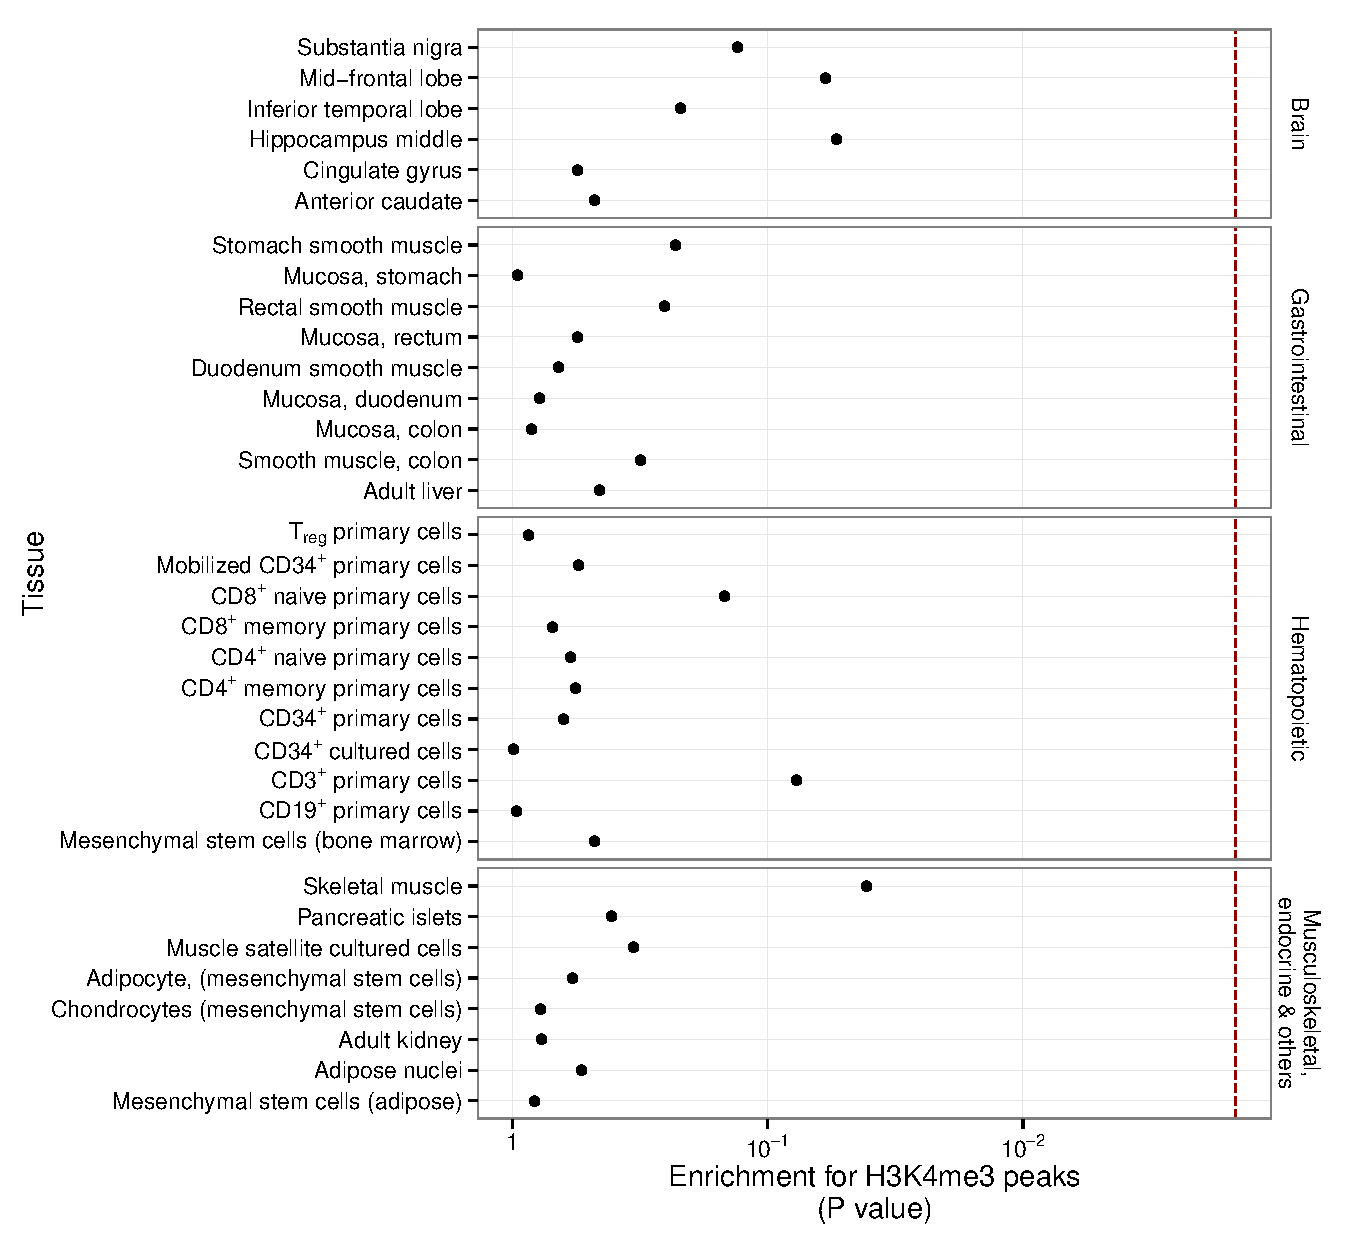
\includegraphics[width=5in]{trans_h3k4me3}
	\caption{\textbf{Tissue specific enrichment of SNPs in transcriptionally active regions} The locations of transcriptional activity can be predicted by chromatin marks, assayed by H3K4me3. Here we show that there is }
	\label{fig:transh3k4me3}
\end{figure}
\clearpage

\begin{figure}
	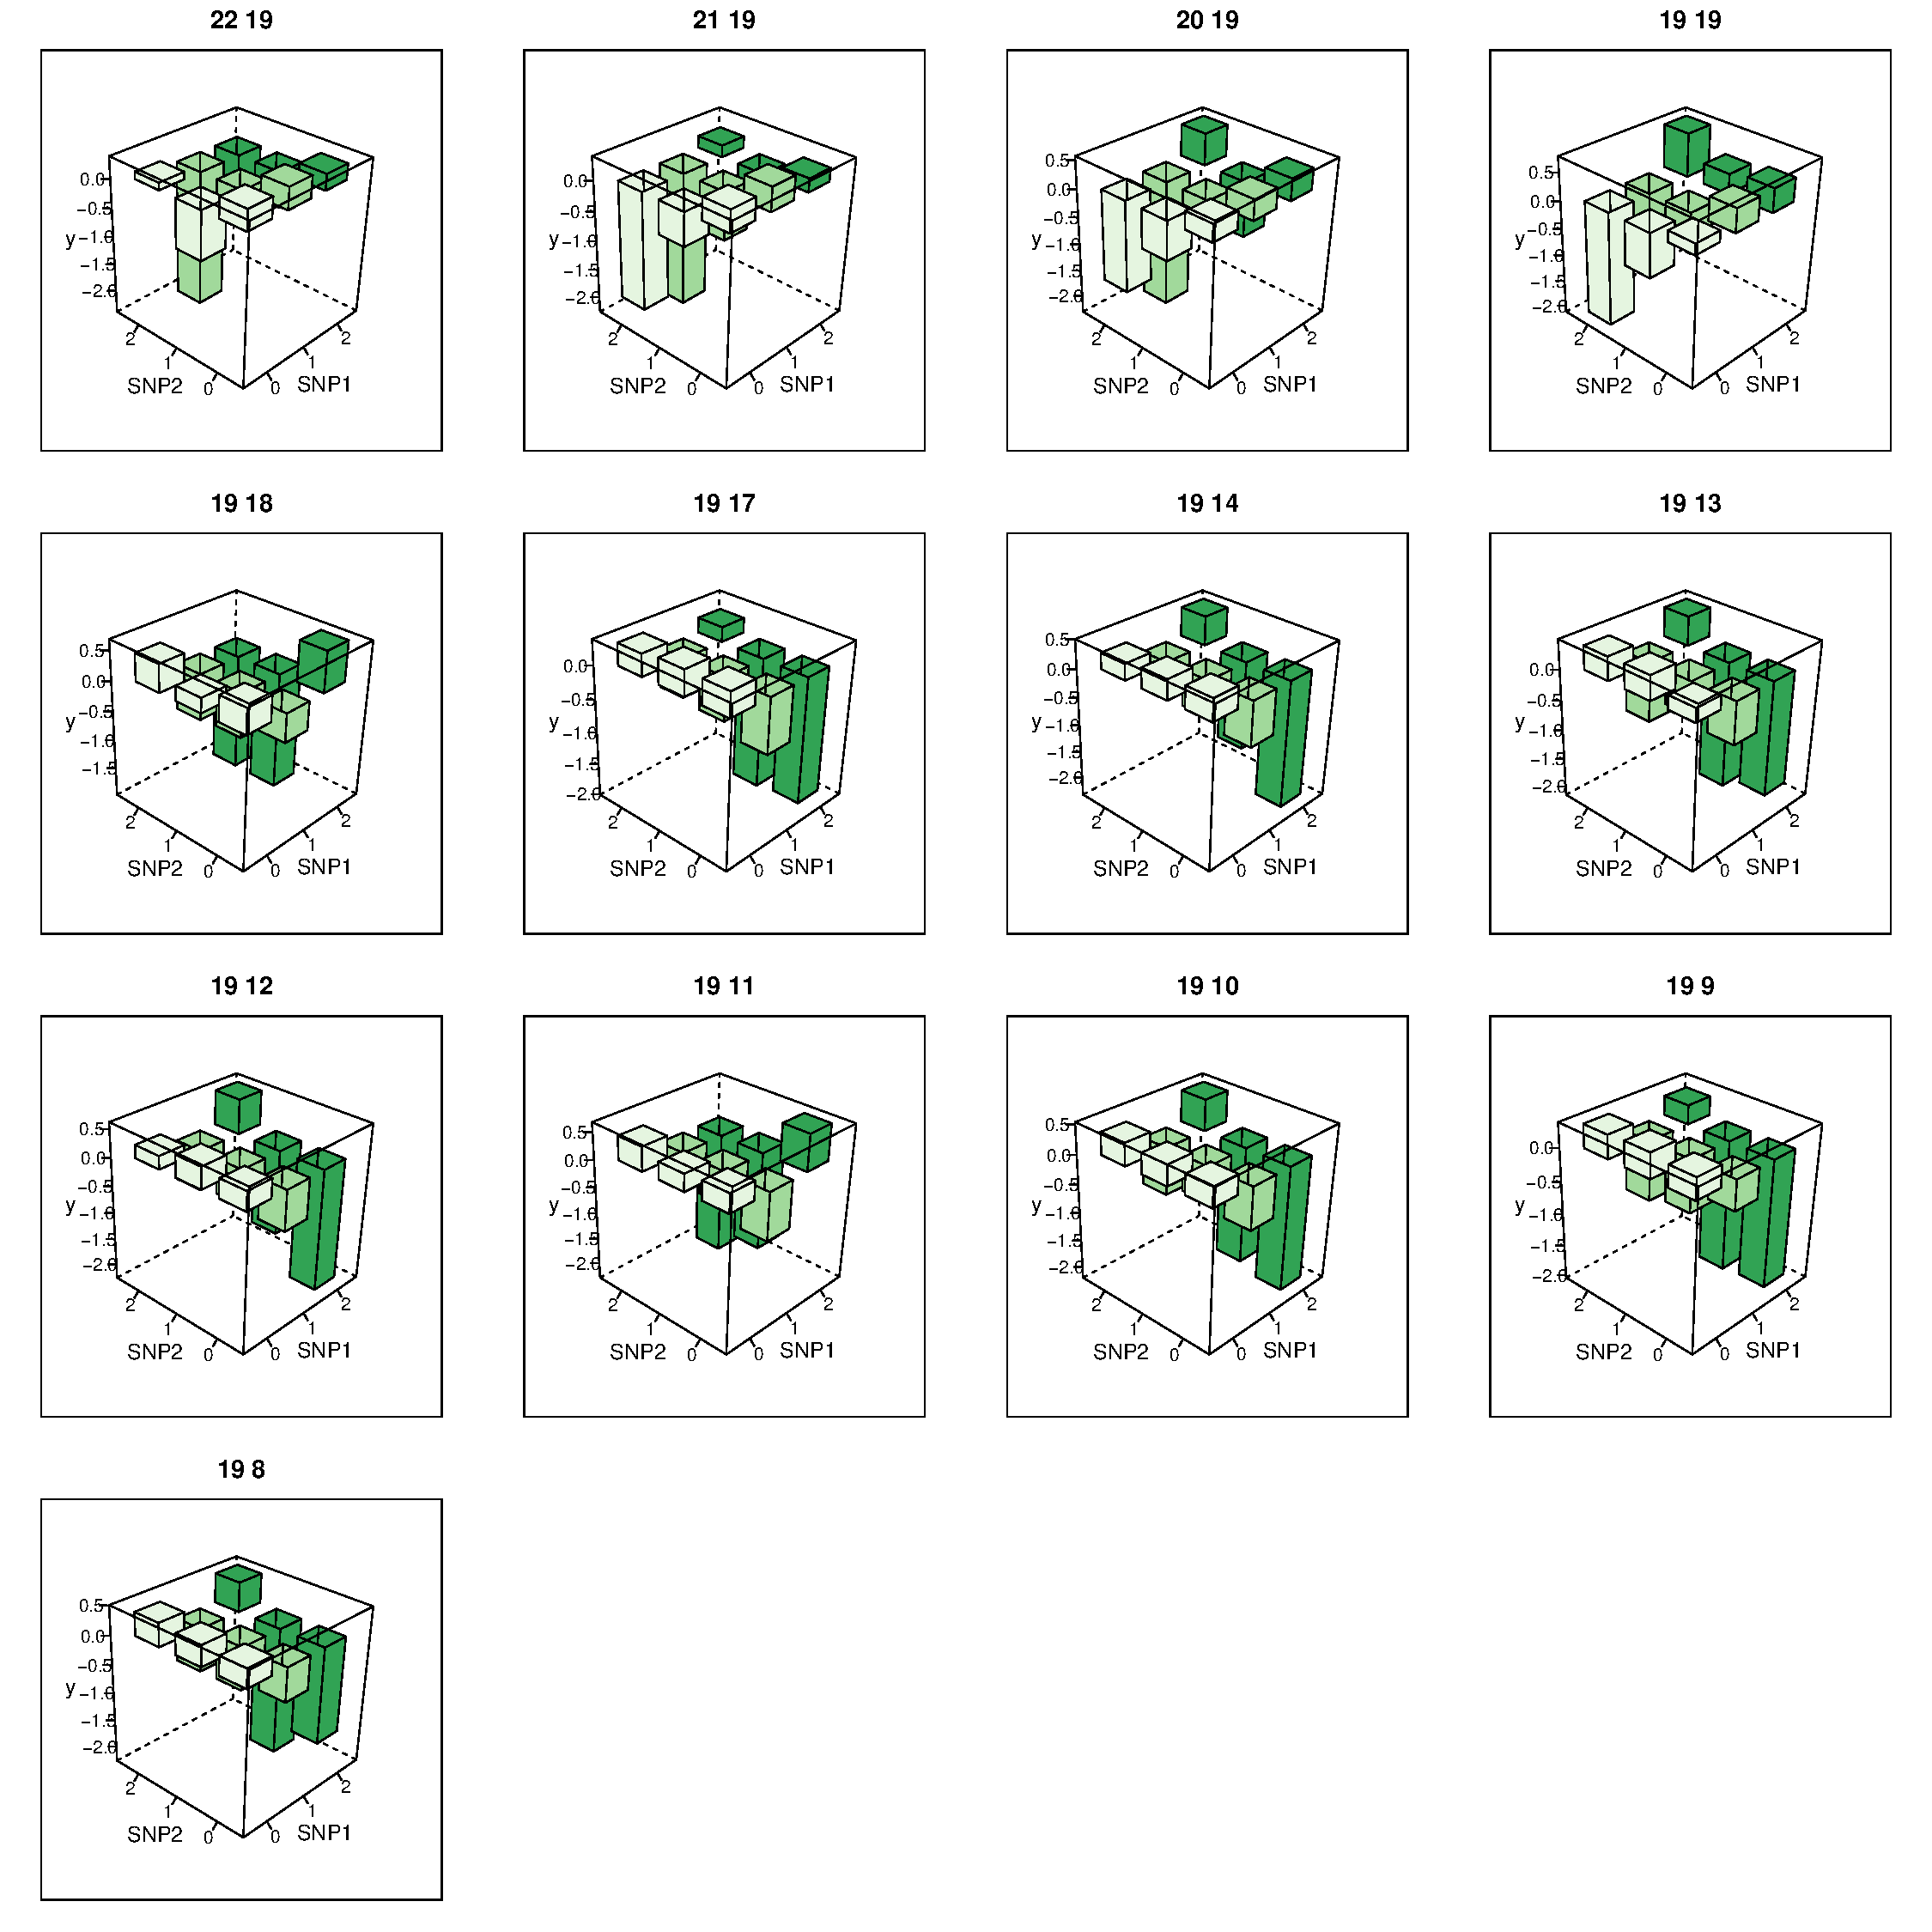
\includegraphics[width=5in]{MBNL1}
	\caption{\textbf{Genotype-phenotype maps for 14 interactions controlling MBNL1} Each bar represents the mean phenotypic value for individuals in that genotype class. The rs13069559 SNP typically has a \emph{cis}-additive decreasing effect on the expression of MBNL1, but in many of these interactions the \emph{cis} effect is masked when the \emph{trans} SNP is homozygous.}
	\label{fig:mbnl13d}
\end{figure}
\clearpage

\begin{figure}
	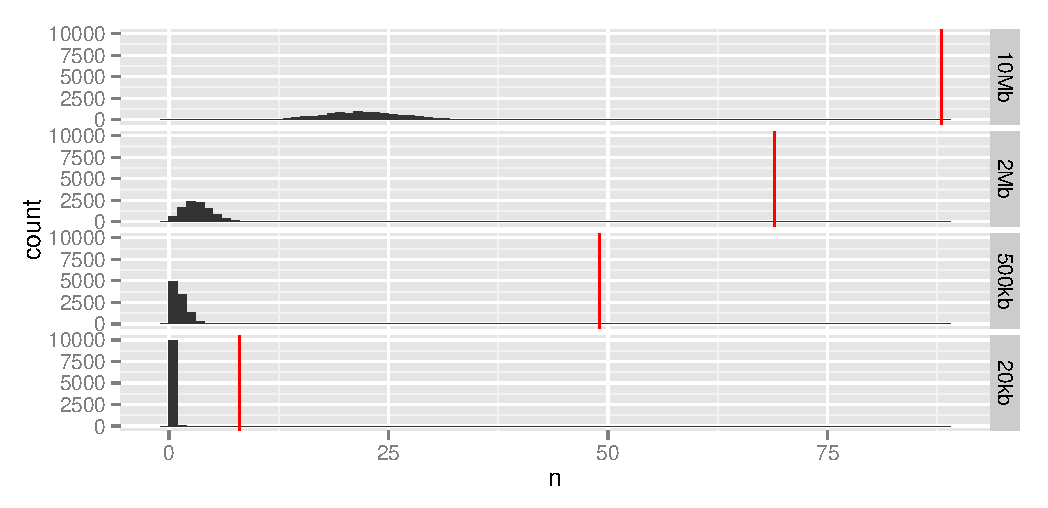
\includegraphics[width=5in]{chromosome_interactions}
	\caption{\textbf{Number of overlaps between chromosome interactions and epistatic interactions} Interacting chromosome regions may be a possible mechanism underlying epistatic interactions. The number of epistatic interactions within 20kb, 500kb, 2Mb and 10Mb of known chromosome interacting regions are shown by red vertical lines. The histograms represent the null distribution based on random sampling of 10000 datasets for each window size.}
	\label{fig:chromosomeinteractions}
\end{figure}
\clearpage

\begin{figure}
	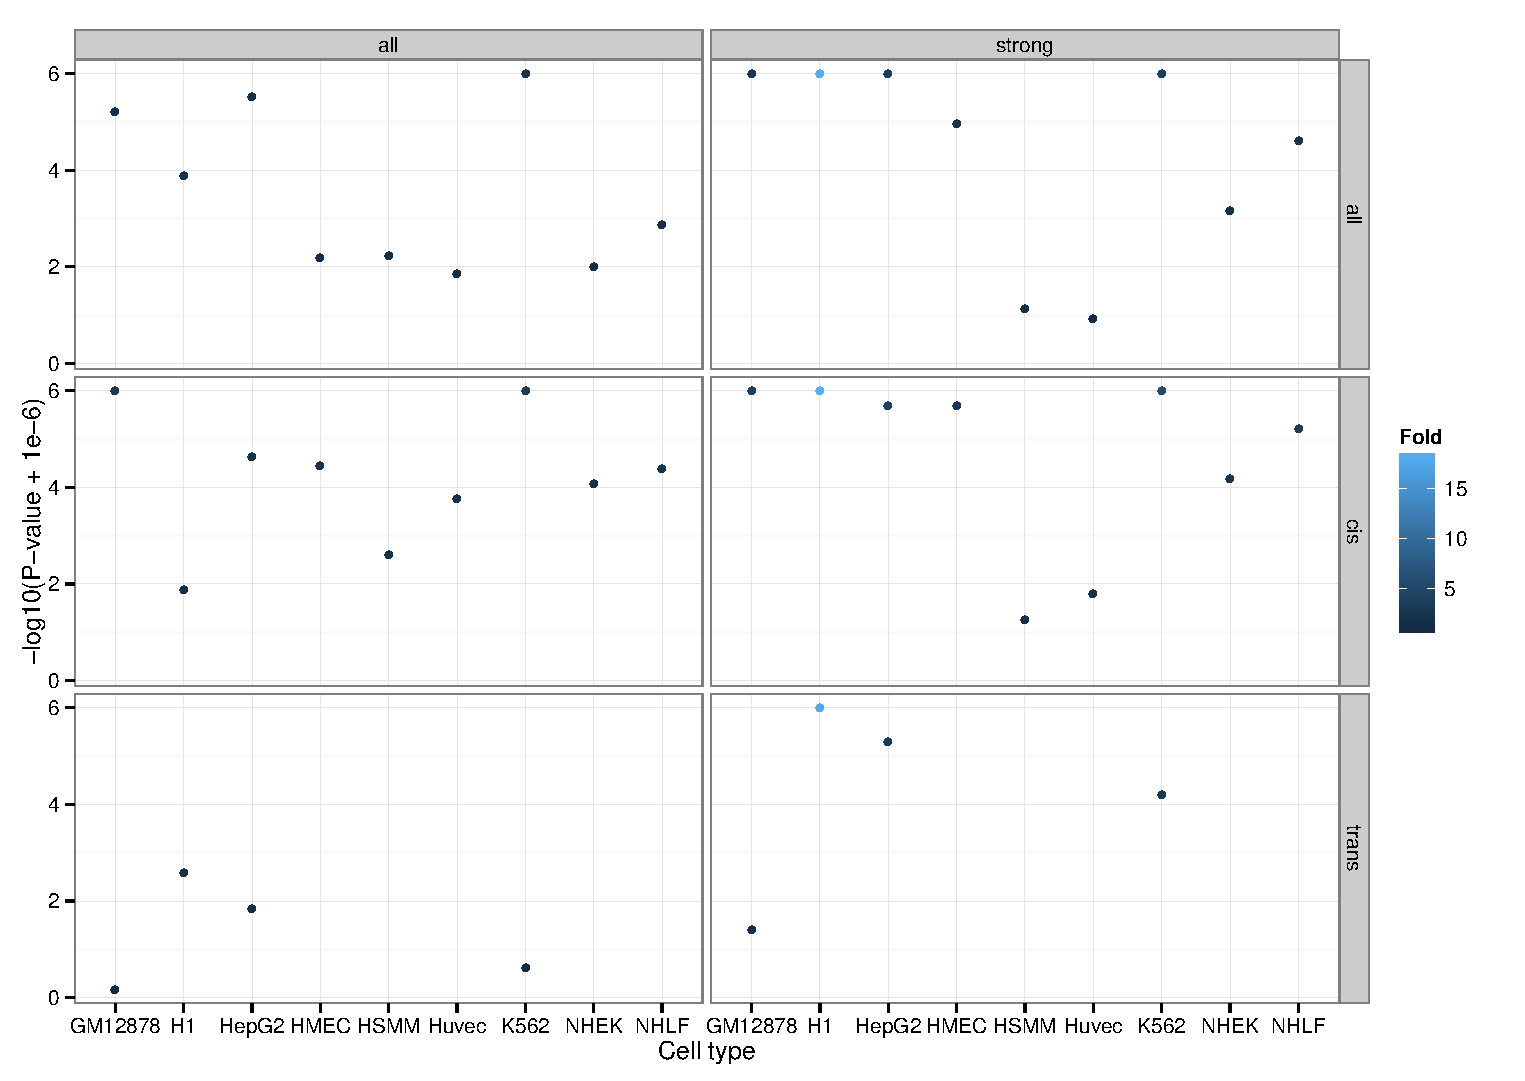
\includegraphics[width=5in]{enhancers}
	\caption{\textbf{There is enrichment for enhancer sequences for \emph{cis} and \emph{trans} SNPs}}
	\label{fig:enhancers}
\end{figure}


\clearpage
\section{References}
\bibliography{refs}

\end{document}